\documentclass{standalone}
\usepackage{tikz}
\usepackage{mathpazo}
\begin{document}

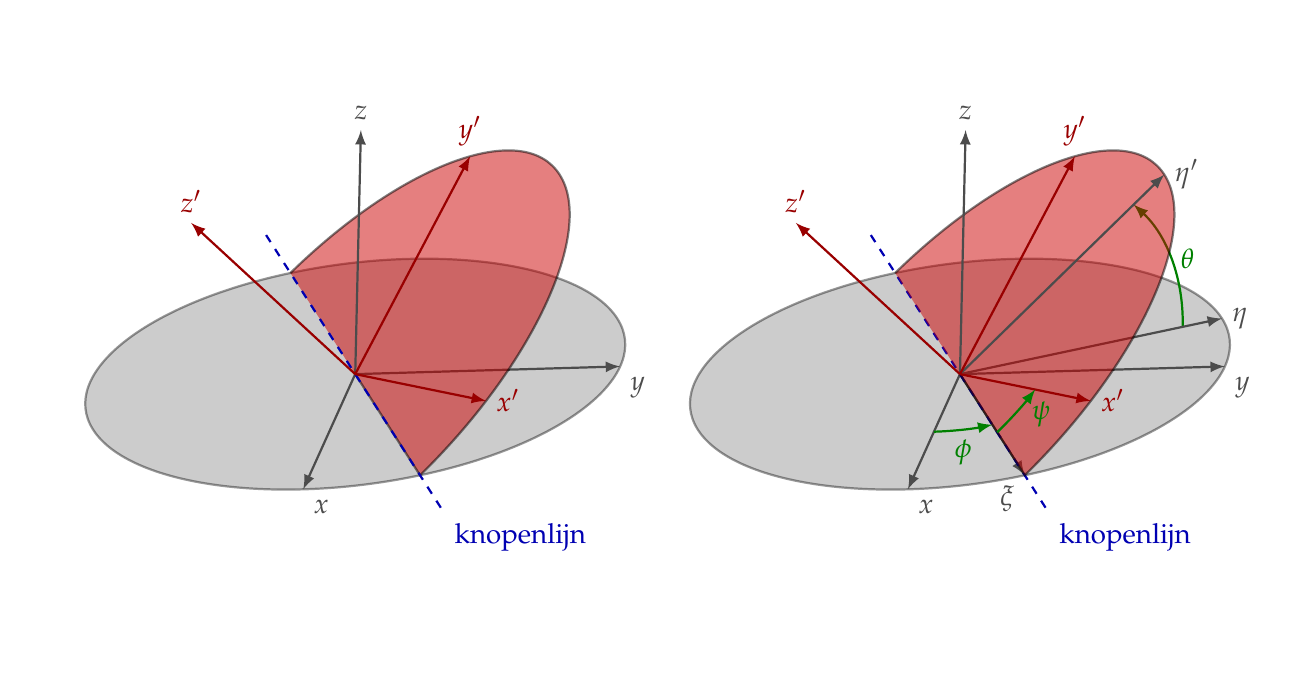
\begin{tikzpicture}[scale=0.8]
\useasboundingbox (-10.0,-4.3) rectangle (10.0,5.5);

% General parameters
\def\radius{4}      % Base plane radius
\def\rA{0.3}        % Small arc radius (for angle indicators)
\def\addAx{0}       % Extra axis length on top of radius (for arrows)
\def\thetaAngle{40} % theta Euler angle
\def\psiAngle{-20}  % psi Euler angle
\def\phiAngle{-25}  % phi Euler angle

\begin{scope}[shift={(-1.2 *\radius,0)}]

  \begin{scope}[rotate around y =-55, rotate around x = -90, rotate around y = 5]

    % Original plane
    \draw[thick, fill=gray,opacity=0.4] (0,0) circle (\radius);
    

    \begin{scope}[rotate around z = \phiAngle]
        % x-axis
        \draw[thick, -latex, color=gray!60!black] (0,0,0) -- (\radius+\addAx,0,0) node[below right] {$x$};

        % y-axis
        \draw[thick, -latex, color=gray!60!black] (0,0,0) -- (0,\radius+\addAx,0) node[below right] {$y$};
      
    \end{scope}

    % red nutation plane
    \begin{scope}[rotate around x = \thetaAngle]
        \draw[thick, fill=red!80!black,opacity=0.5] (0,0,0) -- (\radius,0,0 ) arc (0:180:\radius);
    \end{scope}

    % z-axis
    \begin{scope}[rotate around z = \phiAngle]
        \draw[thick, -latex,color=gray!60!black] (0,0,0) -- (0,0,\radius) node[above] {$z$};
    \end{scope}
    
    % knopenlijn
    \draw[thick,dashed, color=blue!70!black] (-\radius-1.5-\addAx,0,0) -- (\radius+\addAx+1.5,0,0) node[below right] {knopenlijn};


    % Scope of rotated body frame after nutation 
    \begin{scope}[rotate around x = \thetaAngle]
      
      % red nutation plane
      % \draw[fill=red!80!black,opacity=0.5] (0,0,0) -- (\radius,0,0 ) arc (0:180:\radius);

      % final axes (x', y', z')
      \begin{scope}[rotate around z = -\psiAngle]
        
        \draw[thick, -latex, red!60!black] (0,0,0) -- (\radius+\addAx,0,0) node[right] {$x'$};
        
        \draw[thick, -latex, red!60!black] (0,0,0) -- (90-\psiAngle:\radius+\addAx) node[above] {$y'$};
        
        \draw[thick, -latex, red!60!black] (0,0,0) -- (0,0,\radius+\addAx) node[above] {$z'$};
      \end{scope}
      
    \end{scope}
  \end{scope}
\end{scope}

\begin{scope}[shift={(1.2 *\radius,0)}]

  \begin{scope}[rotate around y =-55, rotate around x = -90, rotate around y = 5]

    % Original plane
    \draw[thick, fill=gray,opacity=0.4] (0,0) circle (\radius);

    % x-axis
    \begin{scope}[rotate around z = \phiAngle]
        % x-axis
        \draw[thick, -latex, color=gray!60!black] (0,0,0) -- (\radius+\addAx,0,0) node[below right] {$x$};

        % y-axis
        \draw[thick, -latex, color=gray!60!black] (0,0,0) -- (0,\radius+\addAx,0) node[below right] {$y$};


        \draw[thick,-latex,color=green!50!black] (0,0) ++(\radius-2,0,0) arc (0:-\phiAngle:\radius-2);
        
        \path (0,0) ++(\radius-2,0,0) arc (0:-0.5*\phiAngle:\radius-2) node[below] {\textcolor{green!50!black}{$\phi$}};
      
    \end{scope}

    \begin{scope}[rotate around y=90]
        \draw[thick,-latex, color=green!50!black] (0,0,0) ++(90:\radius-0.6)  arc (90:90+\thetaAngle:\radius-0.6);
        
        \path (0,0,0) ++(90:\radius-0.6)  arc (90:90+0.5*\thetaAngle:\radius-0.6) node[right] {\textcolor{green!50!black}{$\theta$}};
    \end{scope}

    % xi axis
    \draw[thick, -latex,color=gray!60!black] (0,0,0) -- (\radius+\addAx,0,0) node[below left] {$\xi$};

    \draw[thick,dashed, color=blue!70!black] (-\radius-1.5-\addAx,0,0) -- (\radius+\addAx+1.5,0,0) node[below right] {knopenlijn};

    

    % eta axis
    \draw[thick, -latex, color=gray!60!black] (0,0,0) -- (0,\radius+\addAx,0) node[right] {$\eta$};

    % red nutation plane
    \begin{scope}[rotate around x = \thetaAngle]
        \draw[thick, fill=red!80!black,opacity=0.5] (0,0,0) -- (\radius,0,0 ) arc (0:180:\radius);
    \end{scope}

    % z-axis
    \begin{scope}[rotate around z = \phiAngle]
        \draw[thick, -latex,color=gray!60!black] (0,0,0) -- (0,0,\radius) node[above] {$z$};
    \end{scope}

    % Scope of rotated body frame after nutation 
    \begin{scope}[rotate around x = \thetaAngle]

        % eta axis
      \draw[thick, -latex,color=gray!60!black] (0,0,0) -- (0,\radius+\addAx) node[right] {$\eta'$};
      
      % red nutation plane
      % \draw[fill=red!80!black,opacity=0.5] (0,0,0) -- (\radius,0,0 ) arc (0:180:\radius);

      % final axes (x', y', z')
      \begin{scope}[rotate around z = -\psiAngle]
        
        \draw[thick, -latex, red!60!black] (0,0,0) -- (\radius+\addAx,0,0) node[right] {$x'$};
        
        \draw[thick, -latex, red!60!black] (0,0,0) -- (90-\psiAngle:\radius+\addAx) node[above] {$y'$};
        
        \draw[thick, -latex, red!60!black] (0,0,0) -- (0,0,\radius+\addAx) node[above] {$z'$};
      \end{scope}

      % psi indicator
      \draw[thick,-latex,color=green!50!black] (0,0) ++(\radius-1.7,0,0) arc (0:-\psiAngle:\radius-1.7);
      \path (0,0) ++(\radius-1.5,0,0) arc (0:-0.5*\psiAngle:\radius-1.5) node[right] {\textcolor{green!50!black}{$\psi$}};
      
    \end{scope}
  \end{scope}
\end{scope}
\end{tikzpicture}
\end{document}
